\chapter[*合成数据生成]{*用于训练智能体大语言模型的合成数据生成}\label{chap:synthetic-data}


\begin{learningbox}
本章将介绍合成数据（synthetic data）在智能体大语言模型开发中能够发挥的作用。
具体而言，学完本章后，你将能够：
\begin{itemize}[leftmargin=*, nosep]
    \item 阐述{\em 数据}在大语言模型训练流程中的重要性。
    \item 解释从更强模型向较弱学生模型{\em 蒸馏知识}的一般循环。
    \item 描述哪些{\em 流程组件}正在使用合成数据替代人类生成内容。
    \item 概述{\em 整理与评估}合成数据的各种策略。
    \item 通过描述使用人工生成数据的{\em 风险}，比较使用合成数据的优点与缺点。
\end{itemize}
\end{learningbox}

\section{数据的重要性}
大语言模型的快速扩展带来了对训练与评估数据的巨大需求。有人将训练数据称为{\em 数字石油（digital oil）}，以此体现它作为人工智能开发主要原料的重要性。此外，随着训练流程中的模型架构等其他组件日趋同质化，数据正越来越多地成为拉开差距的因素 \citep{11072851}。模型持续扩展，需要从互联网上抓取数万亿词的人类生成文本；然而，可用的人类生成数据总量有限，因此，训练数据是否会成为扩展的主要瓶颈，是一个值得关注的问题，见图~\ref{fig:data-stock} \citep{villalobos2024position}。而且，随着数据需求规模增大，多数易于利用的数据来源逐渐耗尽，获取数据所需的成本与时间也越来越难以承受。隐私、版权与偏见问题也促使这一领域将目光从整理网络上的人类生成数据，转向合成数据生成 \citep{liang2022advances}。

\begin{figure}[tb]
    \centering
    \begin{tikzpicture}[x=0.116mm,y=-0.116mm]
  \node[anchor=north west,inner sep=0] at (0,0) {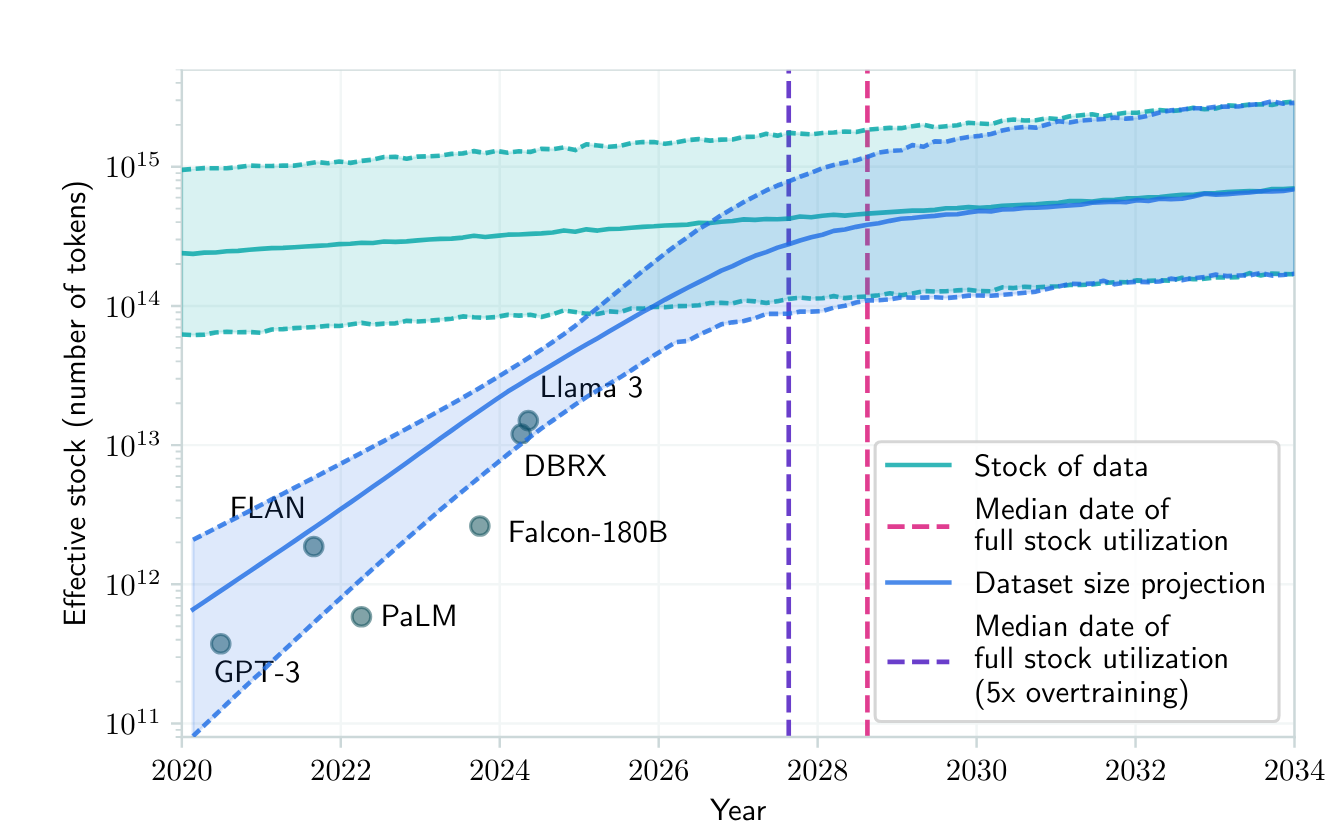
\includegraphics[width=154.976mm]{part6/visuals/data_stock.png}};
  \fill[white] (39,171) rectangle (100,682);
  \node[rotate=90,font=\small,fill=white,inner sep=2pt] at (70,425) {有效存量（词元数）};
  \fill[white] (680,789) rectangle (795,837);
  \node[font=\small] at (739,810) {年份};
  \fill[white] (965,449) rectangle (1269,715);
  \node[anchor=west,font={\fontsize{9}{10.5}\linespread{1}\selectfont}] at (970,467) {数据存量};
  \fill[white] (964,489) rectangle (1270,559);
  \node[anchor=west,align=left,font={\fontsize{9}{10.5}\linespread{1}\selectfont}] at (970,522) {全量数据用尽的\\中位年份};
  \fill[white] (964,565) rectangle (1270,604);
  \node[anchor=west,font={\fontsize{9}{10.5}\linespread{1}\selectfont}] at (970,582) {数据集规模预测};
  \fill[white] (964,607) rectangle (1270,710);
  \node[anchor=west,align=left,font={\fontsize{9}{10.5}\linespread{1}\selectfont}] at (970,657) {全量数据用尽的\\中位年份\\（5 倍超额训练）};
\end{tikzpicture}

    \caption{可用的人类生成公共文本存量与大语言模型训练数据集规模的预测 \citep{villalobos2024position}。存量预测线与数据集规模预测线的交点，表示预计全部存量将被用尽的中位年份（2028 年）。}
    \label{fig:data-stock}
\end{figure}

大语言模型越来越多地自行生成用于训练下一代大语言模型的数据：通过提示，让模型生成指令、对话、推理轨迹，乃至完整的训练语料库，随后用来微调、蒸馏和评估其他模型 \citep{long-etal-2024-llms}。与搜集并标注人类生成文本相比，这种自我强化循环降低了数据收集的成本与工作量，也能精细控制所得数据集的风格、难度与覆盖范围。如今，这种方法已引起产业界 \citep{10.1145/3715275.3732005} 与学术界 \citep{viswanathan-etal-2025-synthetic, alismail2025survey} 的广泛兴趣，其应用涵盖通用指令微调，以及训练工具使用、规划和多步推理等智能体行为所需的更专门的数据（见图~\ref{fig:virtuous}，第 \pageref{fig:virtuous} 页）。

随着对模型生成数据的依赖日益加深，扩展定律（第~\ref{chap:scaling}~章）中也引入了一个新项，用来刻画预训练语料库中合成数据的比例。SYNTHLLM \citep{qin2025scaling} 等近期研究说明了这一点为何重要：它从源文档中自动提取高层概念，再通过基于图的算法重新组合，生成的合成语料足够多样，因而能在不同模型规模下遵循一种可预测的、经修正的扩展定律。在这一版本的扩展定律中，收益会更早趋于平缓，即早于预训练通常采用的其他词元预算；而且，相较于较小模型，较大模型用更少的词元便能达到最优性能。这表明，合成数据不仅可以针对数量进行调节，还可以针对它所形成的扩展曲线形状进行调节。

除了扩展行为，工具使用、规划与多步推理等智能体能力所需的数据生成，也越来越依赖协调的多智能体工作流程，而不是单一生成模型。专门的智能体可以承担不同角色，例如提出任务、执行任务和批评结果，由此产生的数据通常质量更高、更多样，在结构上也更接近智能体训练的实际需求。Matrix \citep{wang2025matrixpeertopeermultiagentsynthetic} 就是这一方向的例子：在这个去中心化框架中，控制流与数据流都表示为通过分布式队列在智能体之间传递的消息，使训练流程无须中央协调器就能水平扩展。下面，我们更仔细地考察合成数据训练流程。


\section{蒸馏循环}
\label{sec:distillation}
在智能体大语言模型的训练流程中使用合成数据，遵循图~\ref{fig:synth-pipeline}~所示的一般蒸馏循环（distillation loop）。生成器可以是一个强模型，也可以是多个智能体的编排系统；它利用少量种子数据或真实数据，生成一个庞大的原始合成数据池。随后，对这个数据池进行{\em 整理}（第~\ref{sec:data-cur}~节），再用来训练或{\em 蒸馏}模型。关键在于，所得模型本身可以成为下一轮迭代的生成器。这种自我强化循环的闭合，会给训练稳定性与下游性能带来相当大的风险（也可参见第~\ref{chap:meta}~章关于元学习稳定性的讨论）。

\begin{figure}[tb]
    \centering
    \resizebox{\linewidth}{!}{
    \begin{tikzpicture}[
        node distance=5mm,
        box/.style={draw, rounded corners=2pt, align=center, minimum height=13mm, minimum width=20mm, font=\footnotesize, thick},
        data/.style={box, fill=blue!8},
        proc/.style={box, fill=orange!12},
        model/.style={box, fill=yellow!14},
        arr/.style={-{Stealth[length=2.5mm]}, thick},
    ]
        \node[data] (seed) {种子数据／\\真实数据};
        \node[proc, right=of seed] (gen) {生成器\\[-1pt]{\scriptsize 教师／多智能体}};
        \node[data, right=of gen] (raw) {原始\\合成数据};
        \node[proc, below=9mm of raw] (inst-eval) {（内在）\\评估};
        \node[proc, right=of raw] (cur) {数据整理\\[-1pt]{\scriptsize 过滤、评分、去重}};
        \node[proc, right=of cur] (train) {训练／\\蒸馏};
        \node[model, right=of train] (model) {模型\\（学生）};
        \node[proc, below=9mm of model] (eval) {（外在）\\评估};
        \foreach \a/\b in {seed/gen, gen/raw, raw/cur, cur/train, train/model}
            \draw[arr] (\a) -- (\b);
        \draw[arr] (model) -- (eval);
        \draw[arr] (raw) -- (inst-eval);
        \draw[arr, dashed] (model.north) -- ++(0,6mm) -| (gen.north)
            node[pos=0.25, above, font=\scriptsize] {改进后的模型成为下一代教师};
    \end{tikzpicture}
    }
    \caption{贯穿本章的合成数据循环。生成器从一个小规模种子集生成原始合成数据，随后进行数据整理、过滤与评分。这些数据用于训练或蒸馏模型，模型经过评估后，可以作为下一轮迭代的生成器（虚线）。}
    \label{fig:synth-pipeline}
\end{figure}

蒸馏（distillation）是合成数据生成的一种特殊情形：生成器是一个{\em 更强的模型，而我们希望迁移它的能力}。在知识蒸馏（knowledge distillation）中，一个紧凑的{\em 学生}模型学习模仿能力更强的{\em 教师} \citep{hinton2015distilling, hu2022teacherstudentarchitectureknowledgelearning}。它既可以直接针对教师的输出预测进行优化，也可以仅在教师生成的合成数据上训练。蒸馏的目标是，在不过多牺牲任务性能的前提下，得到一个在推理阶段与数据成本方面都更高效的教师模型版本。蒸馏已得到广泛应用，也包括智能体场景 \citep[例如，][]{li2025chainofagentsendtoendagentfoundation, du-etal-2025-agentic}。蒸馏还可以用来为指令微调构造偏好数据。例如，Zephyr \citep{tunstall2024zephyr} 使用人工智能反馈进行训练，由强大的教师模型生成输出并排序，以尽量低的数据和训练成本，使一个小模型与用户意图对齐。

\paragraph{蒸馏的四个维度}
具体的蒸馏方法可以沿四个维度来组织。
(1) {\em 信号}：学生模仿的是教师的 logit、完整输出序列，还是由教师给出的标量奖励。
(2) {\em 数据来源}：被评分的序列是由教师生成，还是从学生采样得到。
(3) {\em 时机}：这些数据是在训练前一次性生成（离策略），还是随着学生的变化持续生成（同策略）。
(4) {\em 教师身份}：教师是一个更强的独立模型，还是学生自身。

下面，我们讨论这四个蒸馏维度。

\subsection{信号：蒸馏目标}
如果我们能够以{\em 白盒（white-box）}方式访问教师（$q$）的概率，就可以训练学生 $p_\theta$，使其下一个词元的分布与教师匹配。在蒸馏中，我们经常用相同的温度 $\tau$ 软化这两个分布（即 $q^{\tau}(\cdot) \propto \exp(z/\tau)$，其中 $z$ 为 logit）。在一个序列语料库上，通用蒸馏损失为

\begin{equation}
    \mathcal{L}(\theta) = \mathrm{E}_{x}\left[ \sum_{t} D\big( q^{\tau}(\cdot \mid x_{<t}) \,\|\, p^{\tau}_\theta(\cdot \mid x_{<t}) \big) \right],
    \label{eq:kd}
\end{equation}
其中，对词元位置 $t$ 求和，$D$ 是一种散度（最常用的是 KL 散度），温度 $\tau > 1$ 使两个分布更平缓，从而让学生也能从教师的{\em 相对}置信度中学习。如果只能获得教师的{\em 文本}，也就是{\em 黑盒（black-box）}蒸馏，这通常是通过专有 API 进行蒸馏时的情形，那么我们就无法观测 $q$，而只能获得从中采样的一些词元。此时，软目标 $q^{\tau}(\cdot \mid x_{<t})$ 退化为采样词元对应的独热向量，散度 $D$ 变为词元级交叉熵，式~\ref{eq:kd}~也就化为在教师生成结果上进行的普通监督微调。第~\ref{sec:sim-hum}~节将讨论 Self-Instruct 技术 \citep{wang-etal-2023-self-instruct}。这类方法从数据侧进行蒸馏，因此属于黑盒方法。


\subsection{数据来源：教师—学生范式}
对于蒸馏，一个直观的假设是：教师越大、越强，就总是越好。然而，情况也有例外 \citep{xu-etal-2025-stronger, li-etal-2025-small-models}。能力强的教师可能生成过长、过于复杂，或风格不匹配的轨迹，使小型学生模型难以吸收。这种现象称为{\em 小模型可学习性鸿沟（small model learnability gap）}。图~\ref{fig:small-model-learnability}~展示了一种情形：与前沿模型的复杂思维链相比，小型学生模型从较弱教师的简短推理中学到的更多。其实际启示是，选择教师时应参照学生当前的能力，而不是孤立地追求最强教师 \citep{zhang-etal-2026-find}。

\begin{figure}[tb]
    \centering
    \begin{tikzpicture}[x=0.142mm,y=-0.142mm]
  \node[anchor=north west,inner sep=0] at (0,0) {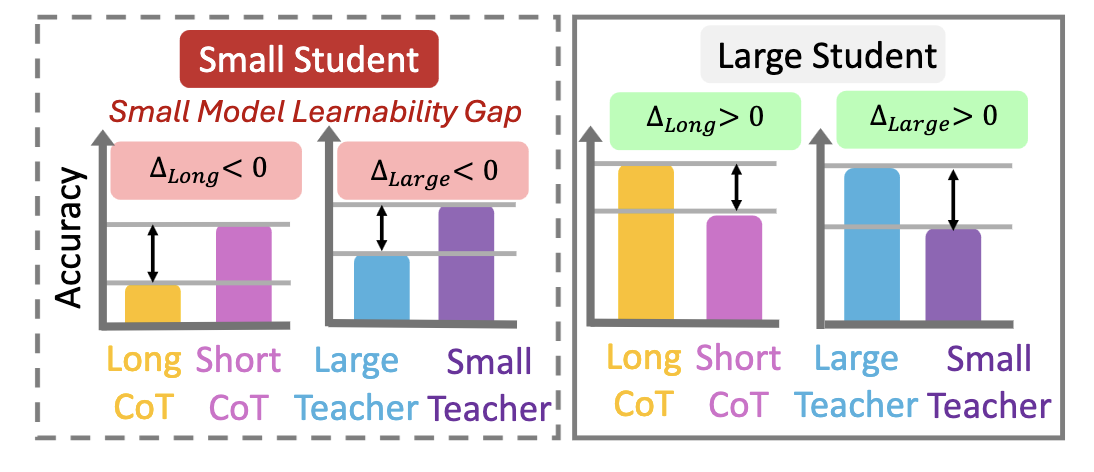
\includegraphics[width=155.348mm]{part6/visuals/student_learner.png}};
  \fill[red!80!black,rounded corners=3pt] (181,32) rectangle (437,87);
  \node[text=white,font=\small\bfseries] at (309,59) {小型学生模型};
  \fill[white] (106,94) rectangle (538,123);
  \fill[white] (106,121) rectangle (317,133);
  \fill[white] (340,121) rectangle (538,133);
  \node[text=red!80!black,font=\small] at (323,111) {小模型可学习性鸿沟};
  \fill[white] (48,159) rectangle (89,313);
  \node[rotate=90,font=\small\bfseries] at (68,237) {准确率};
  \fill[gray!10,rounded corners=3pt] (702,29) rectangle (945,81);
  \node[font=\small\bfseries] at (824,55) {大型学生模型};
  \fill[white] (97,335) rectangle (553,431);
  \fill[white] (599,335) rectangle (1057,431);
  \node[text=orange!90!yellow,align=center,font=\small] at (147,379) {长\\思维链};
  \node[text=magenta!55,align=center,font=\small] at (240,379) {短\\思维链};
  \node[text=cyan!75!blue,align=center,font=\small] at (364,379) {大型\\教师模型};
  \node[text=violet!85!black,align=center,font=\small] at (488,379) {小型\\教师模型};
  \node[text=orange!90!yellow,align=center,font=\small] at (644,379) {长\\思维链};
  \node[text=magenta!55,align=center,font=\small] at (739,379) {短\\思维链};
  \node[text=cyan!75!blue,align=center,font=\small] at (866,379) {大型\\教师模型};
  \node[text=violet!85!black,align=center,font=\small] at (988,379) {小型\\教师模型};
\end{tikzpicture}

    \caption{小模型可学习性鸿沟示意图：小型学生模型并不总能从长思维链推理中受益；使用较小教师生成的较短思维链推理进行微调，反而能取得更好的表现 \citep{li-etal-2025-small-models}。}
    \label{fig:small-model-learnability}
\end{figure}

\subsection{时机：离策略蒸馏与同策略蒸馏}
第三个维度涉及数据生成的时机。蒸馏中最常见的做法是{\em 离策略（off-policy）}蒸馏：从教师采样，得到一个固定的补全数据集，再用这些数据微调学生，如上面的黑盒情形所示。这种方法简单，而且便于并行，但存在训练与推理不匹配的问题。训练阶段，学生只接触那一批由教师生成的词元序列；部署阶段，它却必须继续生成{\em 自己的}序列，而这些序列可能存在缺陷，也可能不同于训练时见过的序列。这种{\em 曝光偏差（exposure bias）}会沿着较长的智能体轨迹不断累积。

{\em 同策略（on-policy）}蒸馏通过在循环内从学生自身采样序列，并让教师为这些序列评分，来解决这一问题。广义知识蒸馏（Generalized Knowledge Distillation，GKD）利用教师针对这些序列的反馈，在学生自行生成的输出序列上训练学生 \citep{agarwal2024policy}。因此，学生恰好在自己实际访问的状态分布上得到纠正。

这种同策略视角通过模仿学习，明确揭示了蒸馏与强化学习之间的联系。式~\ref{eq:kd}~中每个词元对应的教师散度，充当一种{\em 密集的词元级奖励}。
由此，蒸馏变为一种强化学习形式，其中的奖励信号由教师提供，而不是由稀疏的结果检查器提供 \citep{lu2025onpolicydistillation}。混合方案将这一思路进一步拓展，在强化学习阶段，只在模仿教师有帮助的地方选择性地进行模仿 \citep{zhang2026reinforcementaware}。

\subsection{教师身份：自蒸馏与自我改进}
教师模型与学生模型不必不同。当两者相同时，蒸馏就变成了自我改进：模型生成候选解，保留通过检查的结果，再用这些结果训练。STaR \citep{zelikman2022star} 以这种方式自举提升推理能力：迭代生成推理依据，保留能够得到正确答案的结果，再用这些结果进行微调。

另一种方法是自博弈微调（Self-Play Finetuning，SPIN）\citep{chen2024self}。在这种方法中，模型在多轮迭代中区分自身生成结果与参考数据，无须任何外部教师便能改进对齐。或许令人意外的是，即使没有新的数据来源，{\em 反复}自蒸馏也能在一定限度内带来可测量的收益 \citep{pareek2024understandinggainsrepeatedselfdistillation}。

当候选输出能够以较低成本得到{\em 验证}时，自我改进最为有效。在这种情况下，仍然可以有效引入外部信号。代码与数学问题就是如此，因为它们的解很容易执行与检查。例如，CURE 是一个强化学习框架，其奖励依据模型编写代码与生成单元测试的交互结果，使这两种能力共同演化。这里没有用作监督的真值代码。由于代码易于执行和检查，代码编写者与测试编写者可以作为相互适应的智能体，在困难问题上实现长程优化。自我挑战与自我演化智能体也遵循同一原理：它们自行提出越来越困难的任务，并随时间更新生成策略 \citep{NEURIPS2025_a5a305fa, huang2025r, NEURIPS2025_d38653cd}。




\section{模拟人类生成内容}
\label{sec:sim-hum}
从整理后的人类指令数据，发展到合成生成发挥更核心作用的数据集，或许最能体现这一领域如何逐渐摆脱对自然产生的人类文本的依赖；这些文本既可能直接获取，也可能从网络抓取。下面，我们讨论这些方法。不过，从根本上说，这些方法使用的数据集仍以人类生成数据为基础。

Natural Instructions \citep{mishra-etal-2022-cross} 是一个主要由人类提供数据的资源，包含 61 项不同任务、由人类编写的任务指令，以及 19.3 万个任务实例（输入—输出对）。这些指令收集自现有自然语言处理数据集的说明文档，并统一映射到同一种模式。大语言模型实验表明，在看到示例的同时阅读指令，能够使模型受益，不过，这些模型的表现仍远低于估计的性能上界。

后续研究聚焦于增加不同任务及任务类型的数量 \citep{wang-etal-2022-super}、改变指令长度 \citep{bach-etal-2022-promptsource}，或纳入特别困难的任务 \citep{srivastava2023beyond}。需要强调的是，所有这些元数据集，也就是由数据集构成的数据集，归根结底仍建立在人类基准数据之上：其中每一个样本都是由人编写的。因此，能够在网上免费找到的这类数据，在实际数量上存在上限。

由于这些方法依赖以众包数据集形式提供的大量人类监督，近期研究开始着重生成承担相同作用的合成数据。Unnatural Instructions \citep{honovich-etal-2023-unnatural} 等数据集由此出现：它们只需少量人工劳动，主要通过提示各种大语言模型，收集富有创意且多样的指令。实验表明，使用含有一定噪声的 Unnatural Instructions 数据集训练模型，能够取得与高质量人工整理数据训练出的模型相当的结果，如图~\ref{fig:unnatural}~所示。这表明，对于扩展训练数据集的规模与多样性，机器生成数据能够提供一种比人工劳动更具成本效益的选择。

\begin{figure}[tb]
    \centering
    \begin{tikzpicture}[x=0.103mm,y=-0.103mm]
  \node[anchor=north west,inner sep=0] at (0,0) {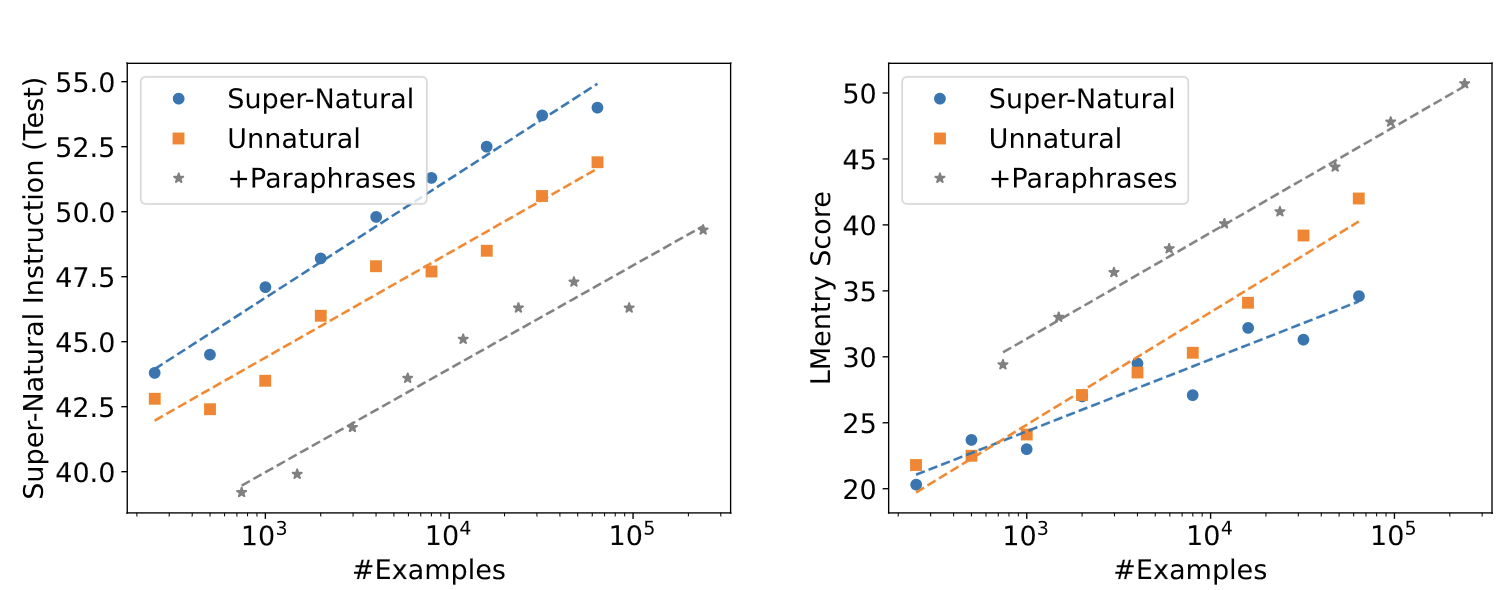
\includegraphics[width=155.118mm]{part6/visuals/unnatural.png}};
  \fill[white] (8,73) rectangle (48,510);
  \node[rotate=90,font=\footnotesize] at (31,291) {Super-Natural Instruction（测试）};
  \fill[white] (797,177) rectangle (839,430);
  \node[rotate=90,font=\footnotesize] at (817,302) {LMentry 得分};
  \fill[white] (217,159) rectangle (421,195);
  \node[anchor=west,font=\footnotesize] at (223,177) {+释义改写};
  \fill[white] (976,158) rectangle (1181,196);
  \node[anchor=west,font=\footnotesize] at (983,177) {+释义改写};
  \fill[white] (337,550) rectangle (529,588);
  \node[font=\footnotesize] at (432,569) {样本数};
  \fill[white] (1097,550) rectangle (1289,588);
  \node[font=\footnotesize] at (1193,569) {样本数};
\end{tikzpicture}

    \caption{比较 Unnatural Instructions 与 Super-Natural Instructions 的扩展实验 \citep{honovich-etal-2023-unnatural}。在控制数据集规模的条件下，分别在 Super-Natural Instructions（左）和 LMentry（右）两个基准测试上评估模型性能。}
    \label{fig:unnatural}
\end{figure}

生成模型对类似人类的文本、代码与推理的模拟，为机器学习系统的训练和评估带来了新方法。通过提示强模型，研究者可以生成高度多样且复杂的数据集，模拟人类生成内容的过程。例如，PersonaHub \citep{ge2025scalingsyntheticdatacreation} 用一个大规模角色设定集合引导生成过程，以这些角色设定提示大语言模型，使其生成的合成数据比无条件生成的数据多样得多。

与自我改进类似，在数学 \citep{NEURIPS2023_44414694, liu2023tinygsmachieving80gsm8k}、编程 \citep{haluptzok2023language} 和游戏 \citep{wang2023voyager} 等模型输出相对容易验证的领域，使用合成数据训练已展现出很大潜力。


\subsection{生成训练数据}
下面，我们聚焦于训练数据的生成。将合成数据用于训练，已经从一种小众的数据增强技术，转变为现代模型对齐与推理流程的核心组件。Self-Instruct \citep{wang-etal-2023-self-instruct} 等技术表明，较小的开放权重模型可以使用完全由更强专有模型生成的数据进行指令微调。如图~\ref{fig:self-instruct}~所示，这个过程以一小组人工编写的指令作为大语言模型的种子，提示它迭代生成新的任务描述、输入与输出。这种模拟的人类内容，无须大批人工标注者，就能让模型获得复杂的零样本能力。

\begin{figure}[tb]
    \centering
    \definecolor{chNineteenTaskBlue}{RGB}{46,84,151}
\begin{tikzpicture}[x=0.110mm,y=-0.110mm]
  \node[anchor=north west,inner sep=0] at (0,0) {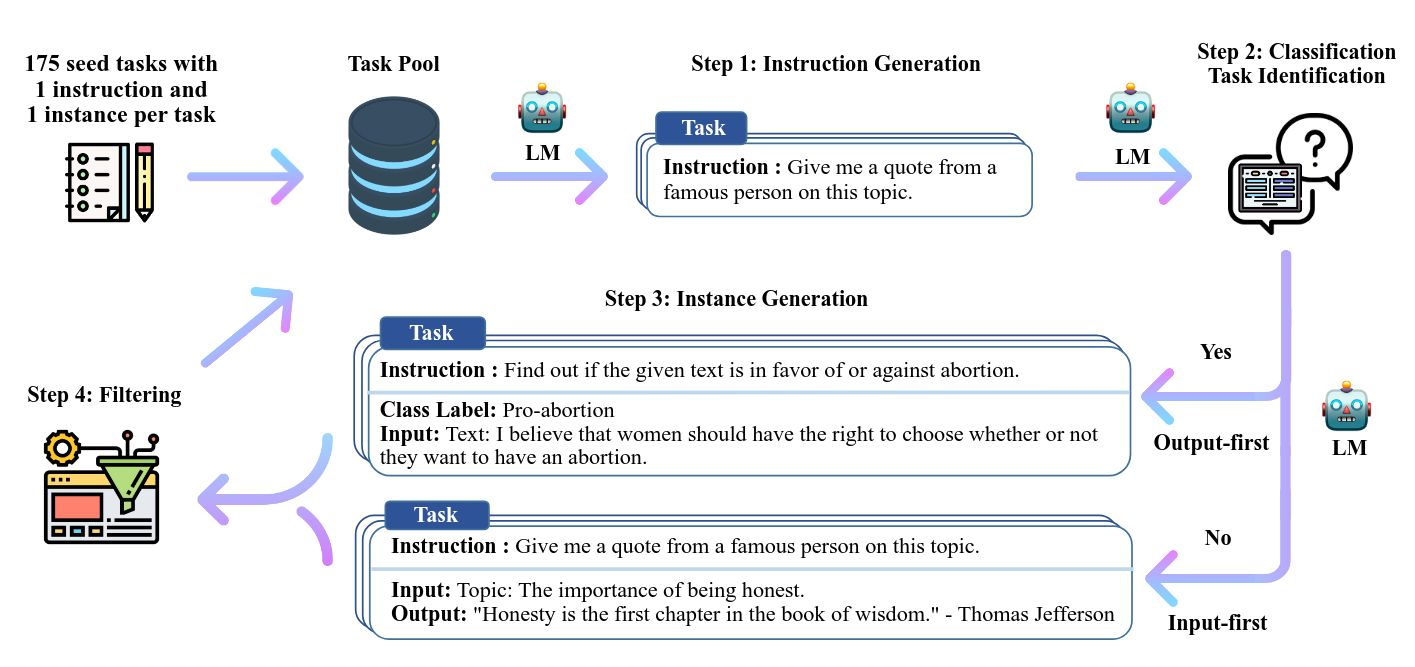
\includegraphics[width=155.65mm]{part6/visuals/self-instruct.png}};
  \fill[white] (16,43) rectangle (245,125);
  \node[align=center,font=\fontsize{8}{9.2}\selectfont] at (129,84) {175 项种子任务\\每项含 1 条指令\\和 1 个实例};
  \fill[white] (342,47) rectangle (457,79);
  \node[font=\footnotesize\bfseries] at (397,63) {任务池};
  \fill[white] (680,42) rectangle (1001,83);
  \node[font=\footnotesize\bfseries] at (838,64) {步骤 1：指令生成};
  \fill[white] (518,139) rectangle (566,165);
  \node[font=\fontsize{7.3}{8}\selectfont] at (542,151) {语言模型};
  \fill[chNineteenTaskBlue] (657,114) rectangle (746,141);
  \node[text=white,font=\fontsize{7.5}{8.5}\selectfont\bfseries] at (702,127) {任务};
  \fill[white] (660,151) rectangle (1027,205);
  \node[anchor=north west,text width=38.8mm,align=left,font=\fontsize{7.5}{8.5}\selectfont,inner sep=0pt] at (664,156) {\textbf{指令：}给我一句有关这一主题的名人名言。};
  \fill[white] (1184,36) rectangle (1413,89);
  \node[align=center,font=\fontsize{8}{9.5}\selectfont\bfseries] at (1294,63) {步骤 2：识别\\分类任务};
  \fill[white] (1109,143) rectangle (1155,168);
  \node[font=\fontsize{7.3}{8}\selectfont] at (1132,155) {语言模型};
  \fill[white] (593,281) rectangle (877,313);
  \node[font=\footnotesize\bfseries] at (736,299) {步骤 3：实例生成};
  \fill[chNineteenTaskBlue] (383,319) rectangle (484,346);
  \node[text=white,font=\fontsize{7.5}{8.5}\selectfont\bfseries] at (433,333) {任务};
  \fill[white] (376,355) rectangle (1123,388);
  \node[anchor=west,font=\fontsize{8}{9}\selectfont,inner sep=0pt] at (380,373) {\textbf{指令：}判断给定文本支持还是反对堕胎。};
  \fill[white] (375,395) rectangle (1123,467);
  \node[anchor=north west,text width=80mm,align=left,font=\fontsize{8}{9.2}\selectfont,inner sep=0pt] at (380,400) {\textbf{类别标签：}支持堕胎\\\textbf{输入：}文本：我认为，女性应有权选择自己是否要堕胎。};
  \fill[white] (1185,335) rectangle (1260,365);
  \node[font=\fontsize{8}{9}\selectfont\bfseries] at (1223,351) {是};
  \fill[white] (1147,426) rectangle (1283,460);
  \node[font=\fontsize{8}{9}\selectfont\bfseries] at (1215,443) {输出优先};
  \fill[white] (1325,433) rectangle (1380,461);
  \node[font=\fontsize{7.3}{8}\selectfont] at (1353,448) {语言模型};
  \fill[chNineteenTaskBlue] (386,503) rectangle (487,529);
  \node[text=white,font=\fontsize{7.5}{8.5}\selectfont\bfseries] at (436,516) {任务};
  \fill[white] (374,532) rectangle (1126,566);
  \node[anchor=west,font=\fontsize{8}{9}\selectfont,inner sep=0pt] at (380,548) {\textbf{指令：}给我一句有关这一主题的名人名言。};
  \fill[white] (374,575) rectangle (1124,631);
  \node[anchor=west,font=\fontsize{7.5}{8.5}\selectfont,inner sep=0pt] at (380,589) {\textbf{输入：}主题：诚实的重要性。};
  \node[anchor=west,font=\fontsize{7.5}{8.5}\selectfont,inner sep=0pt] at (380,615) {\textbf{输出：}“诚实是智慧之书的第一章。”——Thomas Jefferson};
  \fill[white] (1194,521) rectangle (1256,551);
  \node[font=\fontsize{8}{9}\selectfont\bfseries] at (1224,537) {否};
  \fill[white] (1157,605) rectangle (1289,639);
  \node[font=\fontsize{8}{9}\selectfont\bfseries] at (1222,622) {输入优先};
  \fill[white] (14,376) rectangle (202,412);
  \node[font=\fontsize{8}{9}\selectfont\bfseries] at (105,395) {步骤 4：过滤};
\end{tikzpicture}

    \caption{Self-Instruct 流程 \citep{wang-etal-2023-self-instruct}。}
    \label{fig:self-instruct}
\end{figure}

\paragraph{利用现有数据}
另一些方法将整理后的人类数据与合成数据结合起来，而不是用其中一种替代另一种。\citet{gunasekar2023textbooksneed} 表明，将人工编写的教科书与合成文本混合用于训练，能够得到能力出色的语言模型，这说明整理后的人类数据与机器生成数据是互补关系。一个挑战在于，即使以人类生成数据作为种子，合成数据仍往往缺乏多样性，并且会继承错误与幻觉。后续改进采用了基于真值文档的生成过程 \citep{lupidi2025sourcesynth, NEURIPS2024_a4ca07aa}。


另一种扩充有限种子集的互补方法是{\em 回译（backtranslation）}。这种方法最初用于机器翻译：将句子从源语言译成目标语言，再译回源语言，以合成平行数据 \citep{edunov-etal-2018-understanding}。同一原理也可以用于推理任务：除了为单个问题生成具体解答，还可以生成与现有解答一致的新问题。MathGenie \citep{lu-etal-2024-mathgenie} 将这一思路用于数学推理，以问题—解答对的种子集为起点，先扩充解答，再将其回译为新问题。由于每个新生成的问题都以已验证的解答为依据，这种方法能够在减少错误与幻觉的同时，扩大训练数据的规模与多样性。

\paragraph{人在回路中的方法}
完全自动化的生成流程并不总能满足需要。模型可能难以生成特定场景或与领域相关的案例。这些失败通常是因为用于生成的大语言模型存在特定盲区，也因此难以生成确实能提供新信息的数据 \citep{lippmann2024illuminatingblindspotslanguage}。

这些问题推动了{\em 人在回路中（human-in-the-loop）}的方法：人们引导、过滤或修改机器生成内容，而不是从头编写。

WANLI \citep{liu-etal-2022-wanli} 将提出具有挑战性的自然语言推理示例的语言模型，与负责筛选和重新标注这些示例的人工标注者配合起来，把自动生成的可扩展性与人工质量控制相结合。

EvalAssist \citep{santillan-cooper-etal-2025-synthetic} 将类似原理用于评估工具，借助合成数据支持并加快人工判断。一种相关策略是，提示语言模型生成初始种子文本，由人工评分者编辑，再将结果用于自举生成更大规模的全合成数据集。这样，人类的精力就用于纠正模型，而非编写每一个示例。



\subsection{生成评估数据}
除了训练，合成生成在评估中也发挥关键作用。传统静态基准测试面临迅速发生的数据污染问题：测试集会意外泄漏到现代大语言模型的预训练语料库中。为缓解这一问题，动态评估框架 \citep{kiela-etal-2021-dynabench} 越来越多地依靠合成数据生成，创建定制的一次性测试用例。

此外，{\em 大语言模型裁判（LLM-as-a-judge）}范式 \citep{zheng2024judging} 通过提示一个强模型对其他模型的输出评分，来模拟人工评估，使模型评分与人类偏好高度相关，并显著缩短评估周期。

为大语言模型创建专用的高难度基准测试，也可以再次采用人在回路中的方法，例如 MATH$^2$ 基准测试。在该基准中，多个大语言模型通过多轮提示，迭代生成并调整数学问题与解答。人工标注者随后进一步扩展问题并检查答案，在这一过程中同样得到大语言模型的协助 \citep{shah2024ai}。其他高效生成合成评估数据的方法，则将标注者的任务从构思新样本，转为编辑样本，使其对大语言模型而言更难 \citep{yuan2021synthbio}。

\paragraph{自动化红队测试}
机器生成评估数据的一个具体用途，是通过{\em 自动化红队测试（automated red teaming）}开展面向安全的评估。在这种方法中，一个大语言模型生成对抗性提示，在目标模型部署前探测其漏洞 \citep{ganguli2022redteaminglanguagemodels}。通过合成大量潜在恶意提示，研究者可以按人工红队无法企及的规模，对模型开展压力测试，并增强其抵御有害输出、越狱与失对齐问题的能力 \citep{perez-etal-2022-red}。由于随后还可以用同一批生成提示微调目标模型，以应对这些失效问题，红队测试因而处于合成评估数据与合成训练数据的交界处。


\subsection{生成智能体数据}
在智能体场景中，需要为整条轨迹合成数据，而不只是生成单个指令—回答对。智能体与环境交互时，会产生包含工具调用、观测与决策的完整序列 \citep{kang2025distilling}。这超出了训练或评估仅处理单个输入—输出对的常规大语言模型所需的数据。尽管通常使用相同的生成模型，生成智能体数据仍比为底层大语言模型本身生成指令数据更复杂。下面来看一个例子。


\begin{example}
考虑为一个使用工具的智能体合成一条训练轨迹，大体遵循 APIGen-MT 的两阶段方案 \citep{NEURIPS2025_5e3661f7}。

首先，{\em 任务提出者（task proposer）}构想一个合理的用户目标、一组可用工具，以及一个真值答案：

\emph{用户：}“这个周末莱顿的天气怎么样，我应该带伞吗？”\quad \emph{工具：}\texttt{get\_forecast(city, days)}。

随后，一个{\em 行动者（actor）}模型展开交互，发出中间工具调用，读取其（模拟）观测结果，然后作答：

\begin{center}\small
\texttt{get\_forecast("Leiden", 2)} $\rightarrow$ \texttt{\{sat: rain, sun: clear\}} $\rightarrow$ \emph{“周六有雨，周日晴朗——周六请带伞。”}
\end{center}

最后，{\em 验证器（verifier）}检查发出的调用格式是否正确、参数是否符合请求，以及最终回答是否与观测一致。只有通过验证的轨迹才会保留。

请注意，这里需要合成的内容包括目标、工具模式、调用、观测，以及验证整个轨迹的检查器，而不只是单个输入—输出对。
\end{example}

智能体数据生成方法通常涉及对智能体的完整编排，以开展包含人类输入与工具使用的多轮对话 \citep{wu2024autogen}。APIGen-MT \citep{NEURIPS2025_5e3661f7} 用一个两阶段框架生成可验证且多样的多轮智能体数据，体现了这一转变。TOUCAN \citep{xu2025toucansynthesizing15mtoolagentic} 在更大规模上追求类似目标，通过模拟真实的工具调用，构建了一个大型工具使用智能体数据集。除了为固定技能生成轨迹，还有研究专门合成数据，将一种新技能或行为从强模型迁移给较弱模型，这一过程称为生成式教学（Generative Teaching）\citep{crispino2023agent}。此外，智能体合成数据也不限于文本，类似的生成流程还可延伸至图像、表格数据，以及其他形式的交互或行为数据。

生成智能体合成数据时，控制任务复杂度始终是一项挑战。例如，深度研究智能体旨在通过与在线工具进行长程交互，解决复杂的问答任务；然而，通常用于训练它们的数据，缺乏对难度与质量的精细控制，导致合成数据未能充分体现所需的复杂性。\citet{pandit2025synthesizingagenticdataweb} 为解决这一问题，提出了一套合成问答对的流程，逐步增加任务复杂度，直到一个前沿基线网络智能体失败。这种课程学习方法直接以智能体能力校准任务难度，而不是采用固定的启发式规则。

AReaL-SEA \citep{gao2026selfevolvingsyntheticdataverifiablereward} 从互补的角度解决可靠性问题。它使用多智能体引擎合成以工具为依据的对话，并为每个实例配备可执行的检查器。随后，闭环自我演化过程持续更新提示，提高可靠性。



\section{数据整理}
\label{sec:data-cur}

生成合成数据后，需要检查其质量，并进行整理。通常，这意味着过滤、评分和选择样本，只保留有用的示例。评估合成数据的有用性，可以采取两种互补方法：{\em 外在评估}通过衡量数据对下游任务的影响来评估；{\em 内在评估}则直接考察生成数据或生成过程本身的性质。

实践中，数据整理实现为一个多阶段过滤流程，将下面讨论的标准转化为具体操作。典型阶段包括{\em 语义去重（semantic deduplication）}，即通过嵌入相似度删除近重复示例以保留多样性；{\em 困惑度过滤（perplexity filtering）}，即使用参考模型剔除不连贯或偏离分布的文本；基于规则的检查或格式检查；以及{\em 奖励模型评分或裁判评分}，以仅保留高保真样本。开创性的论文 {\em Textbooks Are All You Need} \citep{gunasekar2023textbooksneed} 提醒我们，这一整理步骤的重要性往往不亚于数据量：为保证质量而严格过滤，可能比单纯增加数量更有价值。如果没有这一步，模型很容易学到教师模型的生成痕迹与统计异常。

\subsection{外在评估}
外在评估（extrinsic evaluation）回答一个简单的问题：合成数据是否确实有助于下游任务？这一问题也称为{\em 效用（utility）}。实践中，衡量效用的方法是，使用合成数据单独或与真实数据混合，训练或微调模型，再在留出的真实世界测试集上评估。外在评估是衡量合成数据是否有用的最直接方式。例如，如果加入合成数据后，预训练模型的性能有所提升，例如困惑度表现改善，就可以认为这些数据有用。然而，这也是成本最高的方法：必须完成一次完整训练，才能获得任何信号。如果改变生成过程，或选择另一组数据，就需要重新训练并评估模型。因此，外在评估不适合在生成过程中用于过滤或选择单个示例。


\subsection{内在评估}
内在评估（intrinsic evaluation）转而考察生成结果本身的特征，无须付出下游训练的成本。研究者已提出多个质量维度，用于评估合成文本 \citep{ramesh-etal-2025-synthtexteval}。除了在输出层面评估，还可以直接对生成过程中使用的语言模型进行基准测试 \citep{kim-etal-2025-evaluating}。与检查生成数据相比，这样能够更早、以更低成本获得信号。


\paragraph{数据正确性}
只有在事实与逻辑上都成立，生成的示例才有用。由于合成数据往往来自其他大语言模型，因此会继承生成模型的失效模式，包括虚构事实、推理不一致，或标签与内容不匹配。这些错误随后可能传播到使用它们训练的模型中。正确性通常通过以下方式检查：将生成结果与人工生成标签比较 \citep{long-etal-2024-llms, chim-etal-2025-evaluating}，执行验证，例如使用基于规则的检查器或独立裁判模型 \citep{chen-etal-2025-mastering, yang-etal-2025-longfaith, NEURIPS2024_4b77d5b8}，或对同一输入的多次生成结果进行一致性检查 \citep{NEURIPS2022_639a9a17, seegmiller-etal-2025-flames}。


\paragraph{数据多样性}
创建合成数据的一个关键问题是维持多样性。Logit 抑制与温度采样能够提高数据多样性，但会牺牲数据正确性 \citep{chung-etal-2023-increasing}。多样性也难以衡量：词汇启发式方法，例如 ROUGE，或神经启发式方法，例如基于嵌入的相似度，经常被用作代理指标，但每一种方法都只能刻画数据潜在变化的一部分。

MetaSynth 通过元提示来生成更具多样性的合成数据，应对这一问题。在此过程中，一个语言模型编排多个专家大语言模型智能体，协同生成数据 \citep{riaz-etal-2025-metasynth}。


\paragraph{数据污染}
合成数据面临的一项严重风险是污染 \citep{deng-etal-2024-unveiling, balloccu-etal-2024-leak}。用于生成的大语言模型在过滤不完善的大规模网络数据集上预训练，可能记住基准测试内容，并在收到生成新训练示例的提示时复现这些内容，或给出非常接近的改写。
经过许多步骤后，合成生成的数据会趋近于现有基准测试的数据。这会人为抬高评估分数，例如代码生成基准测试中的情况 \citep{matton-etal-2024-leakage}。对此类泄漏的解决办法应超越简单的精确匹配过滤，还需要对已知基准测试进行 n 元片段重叠搜索、采用成员身份推理式探测 \citep{puerto-etal-2025-scaling, huang-etal-2026-robust}，或使用动态数据集构建流程 \citep{chen-etal-2025-benchmarking-large}。

\paragraph{公平性与偏见}
大语言模型会继承并放大其训练数据中的社会偏见。如果再用这些模型生成合成语料库，就可能进一步延续刻板关联、失衡的人口群体表征，以及不同社会群体之间生成质量不均等的问题 \citep{gallegos2024bias}。对于合成数据，这尤其值得关注，因为这类数据规模庞大，而且往往被直接用作新大语言模型的训练材料。

最后，内在指标只是有用性的代理指标。一个数据集可能在多样性方面得分很高，也可能通过正确性检查，却未能改善外在评估结果，甚至使之变差。词汇与神经多样性启发式方法衡量的是表层变化，可能无法发现真正有影响的冗余，例如重复的推理模式，也可能高估多样性。
此外，正确性检查依赖可信参考、基于规则的验证器或裁判模型。对于开放式或主观性的生成内容，这些条件可能不存在，或并不可靠。因此，更适合将内在评估视为一项额外检查，它并不能真正替代外在评估。




\section{风险}
\label{sec:risks}

到这里应该已经很清楚，使用合成数据训练智能体大语言模型并非没有问题。下面，我们继续讨论与合成数据相关的几项风险，包括模型坍塌、偏差放大、安全与隐私漏洞，以及法律和伦理方面的关切。

\subsection{模型坍塌}
图~\ref{fig:synth-pipeline}~所示循环的突出风险，在于它将自身输出作为输入。{\em 模型坍塌（model collapse）}是一种已得到充分记录的现象：使用递归生成的人工智能数据训练后续各代模型，会使原始分布的多样性消失 \citep{shumailov2024curserecursiontraininggenerated}。稀有事件和低概率的语言细微差别被采样的次数较少，因此每一代模型都会进一步遗忘分布的长尾行为，直到收敛为一个内容重复、集中于高概率情形的模型。一些实验表明，反复在纯合成数据上训练，带来的收益会递减，最终转为负收益 \citep{singh2024beyond}；将语料库集中于少数合成来源，而非广泛来源，也会使所得模型更加脆弱 \citep{schaffelder2025syntheticeggsbasketsimpact}。类似地，从教师蒸馏得到的小型学生模型容易产生幻觉，而且往往无法处理长尾知识 \citep{pmlr-v202-kandpal23a}。更隐蔽的是，模仿教师可能得到一个在{\em 风格}上接近教师、但在{\em 事实性}上落后的学生模型；这种差距通常只有通过针对性的能力基准测试才会显现 \citep{gudibande2023falsepromiseimitatingproprietary}。标准的缓解措施是持续用真实人类数据锚定语料库，避免仅使用合成数据训练。

\subsection{偏差放大}
由于生成模型过度表征训练分布中的主流模式，合成数据往往会截断自然人类话语中多样的长尾视角 \citep{van-der-meer-etal-2024-empirical}。因此，使用这类数据训练的学生，可能呈现教师社会偏见被放大、被夸张后的版本。学生模型会复现刻板关联、失衡的人口群体表征，或不同群体之间生成质量不均等的问题 \citep{gallegos2024bias}。与原始模型输出相比，这一问题在合成数据上更严重，因为数据被大规模生成，并直接用作训练材料，而且循环的每一轮都会叠加前一轮的影响。

\subsection{安全风险}
合成训练数据也伴随安全风险。依赖生成数据，会为恶意污染训练数据引入新的攻击途径。如果教师模型或生成流程的任何阶段遭到入侵，对手就可以发起数据投毒攻击。由于合成语料库通常规模过大，无法穷尽审计，攻击者可以植入隐蔽后门或恶意指令—回答对；它们会一直潜伏，直到在部署后的学生模型中被触发。研究已表明，即使只污染互联网规模语料库中的极小一部分，也切实可行且成本低廉 \citep{carlini2024poisoning}。如果“教师”是一个不受控制的第三方模型，其训练数据与对齐方式均不透明，风险还会进一步增大。

\subsection{隐私保护}
合成生成经常被视为解决数据隐私问题的方法。其思路是，合成数据不包含个人身份信息（personally identifiable information，PII）\citep{dwork2014algorithmic}，却能够反映病历等私有数据的统计性质。

然而，这类数据存在显著的记忆风险。如果生成阶段没有严格的隐私保证，生成模型可能无意间重建其最初训练所用敏感人类数据的精确片段，从而造成泄漏 \citep{274574}。
隐私评估表明，现成的隐私保护方法可能失效 \citep{ramesh-etal-2024-evaluating}。

常见的隐私方法依赖差分隐私（differential privacy）\citep{dwork2006calibrating}。它为生成过程提供一种保证：当数据集中加入或删除一个人的记录时，输出分布的变化幅度受到上界约束。这一上界由隐私预算控制；预算越小，保护越强，但效用损失也越大 \citep{yue-etal-2023-synthetic}。


\subsection{版权与使用条款}
合成数据的吸引力，一部分来自它绕开了抓取互联网规模人类文本时不明确的法律地位；此类抓取已经引发版权诉讼。
美国 2025 年的 {\em Bartz v.\ Anthropic} 和解案就是一个例子。一家地区法院认定，大语言模型训练本身具有{\em 极强的}转换性，因此可能属于合理使用；然而，责任仍源于底层语料库的{\em 获取}方式，即纳入了数十万本盗版书籍。Anthropic 以每部作品约 \$3{,}000 的金额和解，总额约为 15 亿美元；{\em Kadrey v.\ Meta} 等其他案件也存在类似情形。这表明，训练所用的底层数据，正日益受到版权与使用条款方面的审查。

合成数据并不能完全避开这一问题。从专有模型蒸馏还会引发一个不同的问题：多数商业大语言模型 API 的服务条款明确禁止使用其输出训练竞争模型。因此，无论是否涉及版权，黑盒教师生成的数据都可能存在法律问题。2025 年，一些竞争系统被指控使用前沿 API 的输出进行训练，这种矛盾也因此进入公众视野。对于实践者，这意味着，检查{\em 生成器}的许可，与检查它所替代的人类数据的许可同样重要。


\section{结语}
合成数据已从一种小众增强方法，发展为大语言模型训练流程（第~\ref{chap:pipeline}~章）的核心要素，其推动力是人类文本可能成为扩展瓶颈（第~\ref{chap:scaling}~章）。强模型与多智能体编排系统能够模拟指令数据、评估基准测试；近来，还能模拟由工具调用与决策构成的完整智能体{\em 轨迹}（第~\ref{chap:agents}~章与第~\ref{chap:tools}~章）。

由于原始生成结果含有噪声，数据整理、外在效用，以及对正确性、多样性与污染的内在检查，与生成本身同样重要。各种设置可以视为不同形式的知识蒸馏，沿着信号、数据来源、时机（离策略与同策略）和教师身份这些维度组织起来。

重复使用同一模型的合成数据进行自我改进，有望支持可验证的推理（第~\ref{chap:reasoning}~章）。然而，在所有这些流程中，都必须仔细考察模型使用了什么数据：如果没有真实数据锚定与细致审计，模型坍塌、偏差放大、安全、隐私与许可风险就会随着每次迭代不断累积。

\bibliographystyle{plainnat}
\bibliography{agenticbook,refs,case,synthetic}
